%% Supplementary Information for
%% "From Codes to Causes: A Causal Interpretability Audit of Quantized Delta
%%  Representations in a Transformer World Model"
%% Standalone; compile: tectonic sn-supplementary.tex
\documentclass[11pt]{article}
\usepackage[margin=1in]{geometry}
\usepackage{graphicx}
\usepackage{booktabs}
\usepackage{amsmath,amssymb}
\usepackage{xcolor}
\usepackage[hidelinks]{hyperref}
\usepackage{textcomp}

\newcommand{\deltairis}{$\Delta$-IRIS}
\newcommand{\code}[2]{(s_{#1},c_{#2})}
\newcommand{\achname}[1]{\texttt{#1}}

\renewcommand{\thefigure}{S\arabic{figure}}
\renewcommand{\thetable}{S\arabic{table}}
\renewcommand{\figurename}{Supplementary Figure}
\renewcommand{\tablename}{Supplementary Table}
\setcounter{secnumdepth}{0}

\title{Supplementary Information\\[2pt]\large From Codes to Causes: A Causal Interpretability Audit of Quantized Delta Representations in a Transformer World Model}
\author{R.\ Xia}
\date{}

\begin{document}
\maketitle

This document collects the displays deferred from the main text: codebook utilisation (Fig.~\ref{sfig:codebook}), the prediction-head read positions (Fig.~\ref{sfig:heads}), single-step ablation (Fig.~\ref{sfig:onestep}), decoded-frame filmstrips (Fig.~\ref{sfig:film}) the partially observed (no-HUD) control (Fig.~\ref{sfig:nohud}), the behavioural cascade test (Fig.~\ref{sfig:cascade}) and the frame-carried-state smoking gun (Fig.~\ref{sfig:hud}); and Tables~\ref{stab:mi}--\ref{stab:logit}: detector codes, cross-corroborated dictionary features, matched-protocol reconstruction, HUD-shortcut margins, the sparse-autoencoder robustness sweep, the empirical random-direction null, steering, and direct logit attribution. All re-use the single frozen agent and the saved rollout corpora described in Methods.

% ---------------- Supplementary Figures ----------------
\begin{figure}[h]
\centering
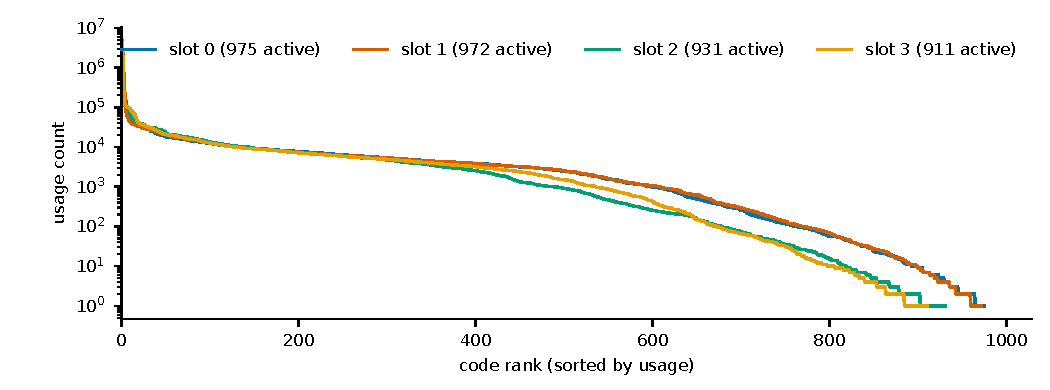
\includegraphics[width=0.9\textwidth]{figures/codebook_usage.pdf}
\caption{\textbf{Codebook utilisation over the full $10^7$-transition replay buffer.} Per-slot code-usage counts, sorted descending (log scale). All 1024 codes are active in the union of slots, but usage is Zipf-like: the head codes encode ``no change in this quadrant'' and the event vocabulary occupies the tail.}\label{sfig:codebook}
\end{figure}

\begin{figure}[h]
\centering
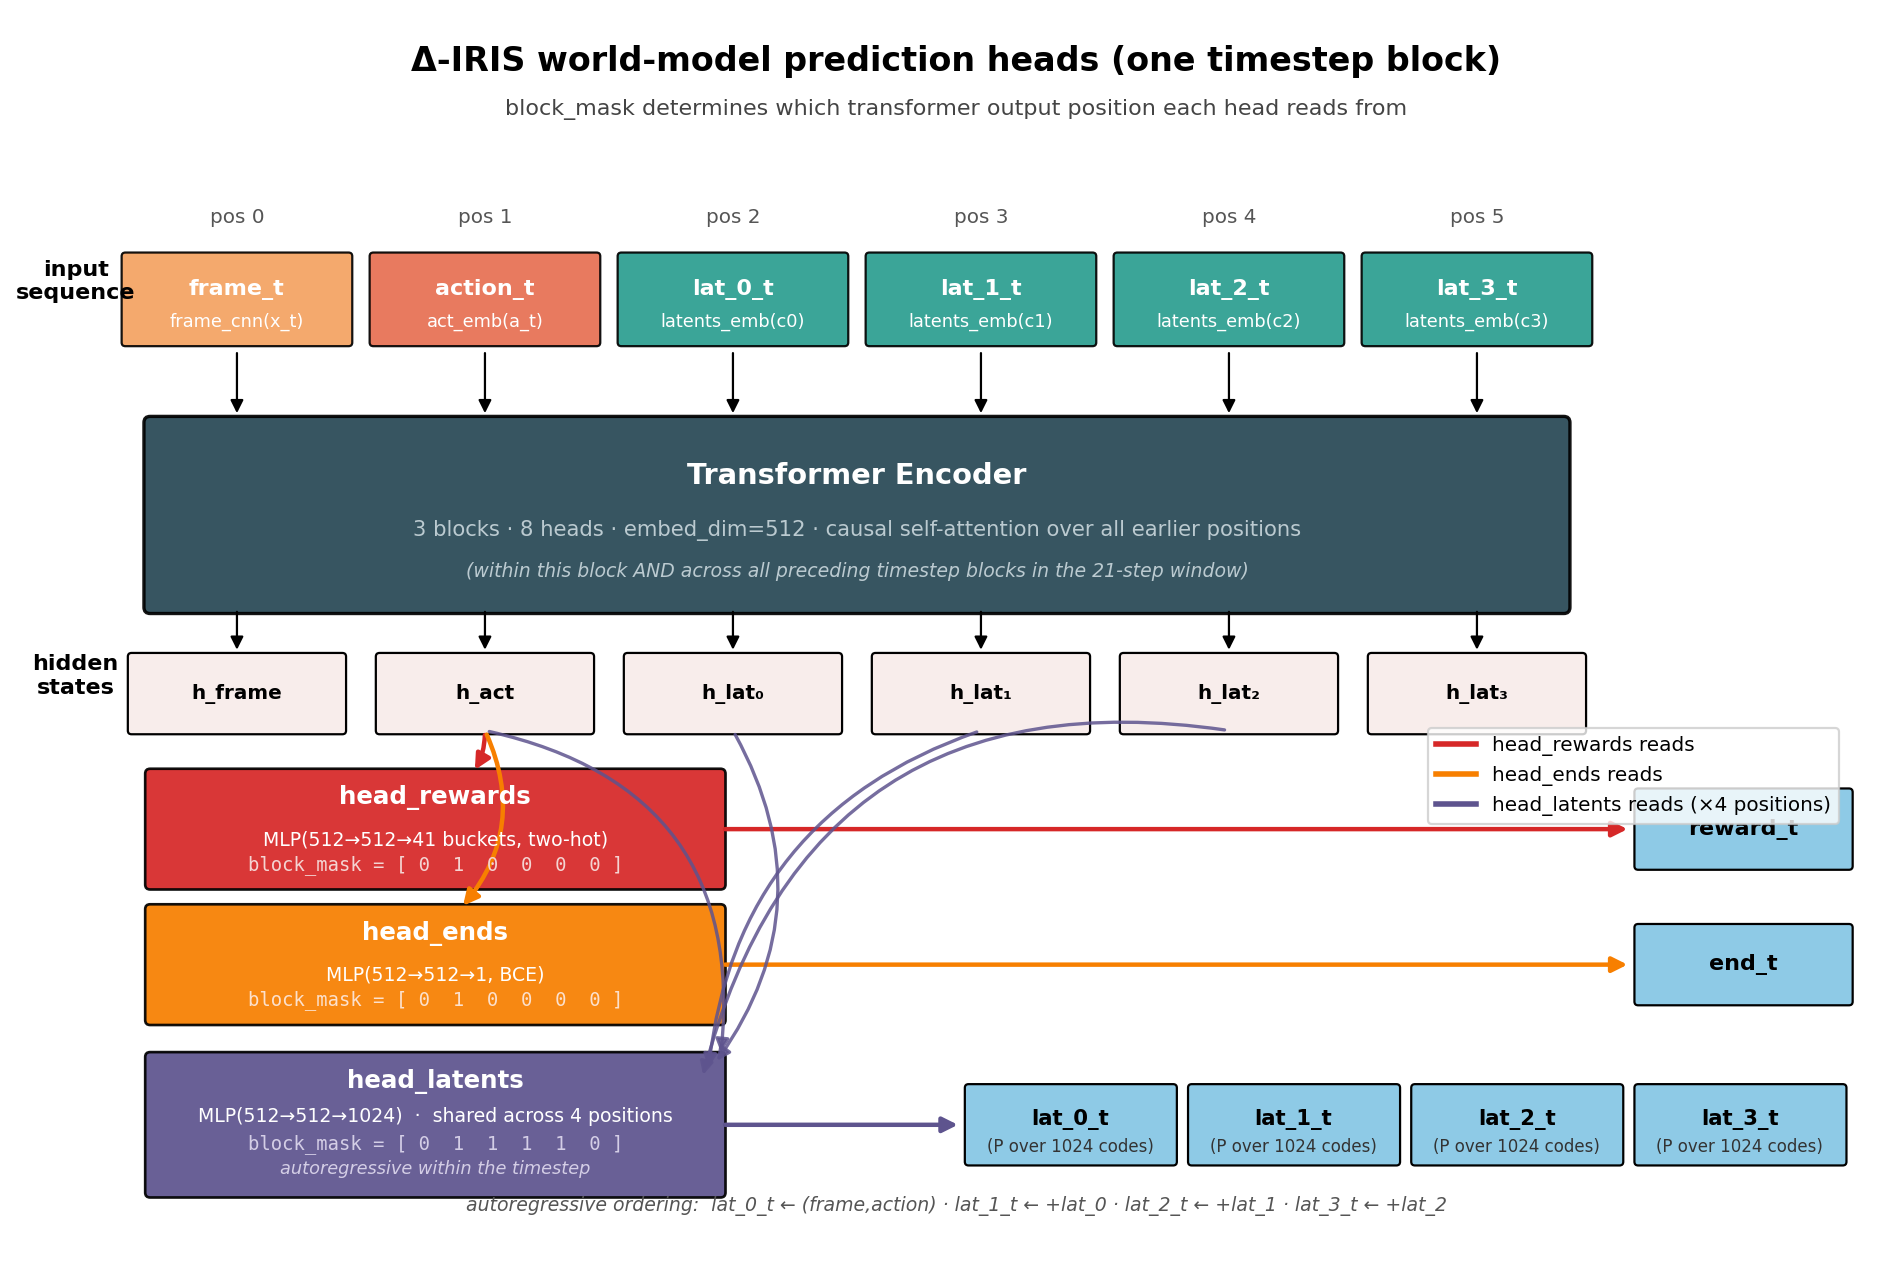
\includegraphics[width=0.85\textwidth]{figures/heads.png}
\caption{\textbf{Detailed view of the \deltairis{} prediction heads} (architecture follows Micheli et al.; our redrawing). \texttt{head\_rewards} and \texttt{head\_ends} read the post-transformer activation at the action position (block mask $[0,1,0,0,0,0]$); \texttt{head\_latents} reads positions 1--4 (mask $[0,1,1,1,1,0]$) and predicts the four latent codes autoregressively within the timestep. The final latent position feeds subsequent attention but carries no prediction head.}\label{sfig:heads}
\end{figure}

\begin{figure}[h]
\centering
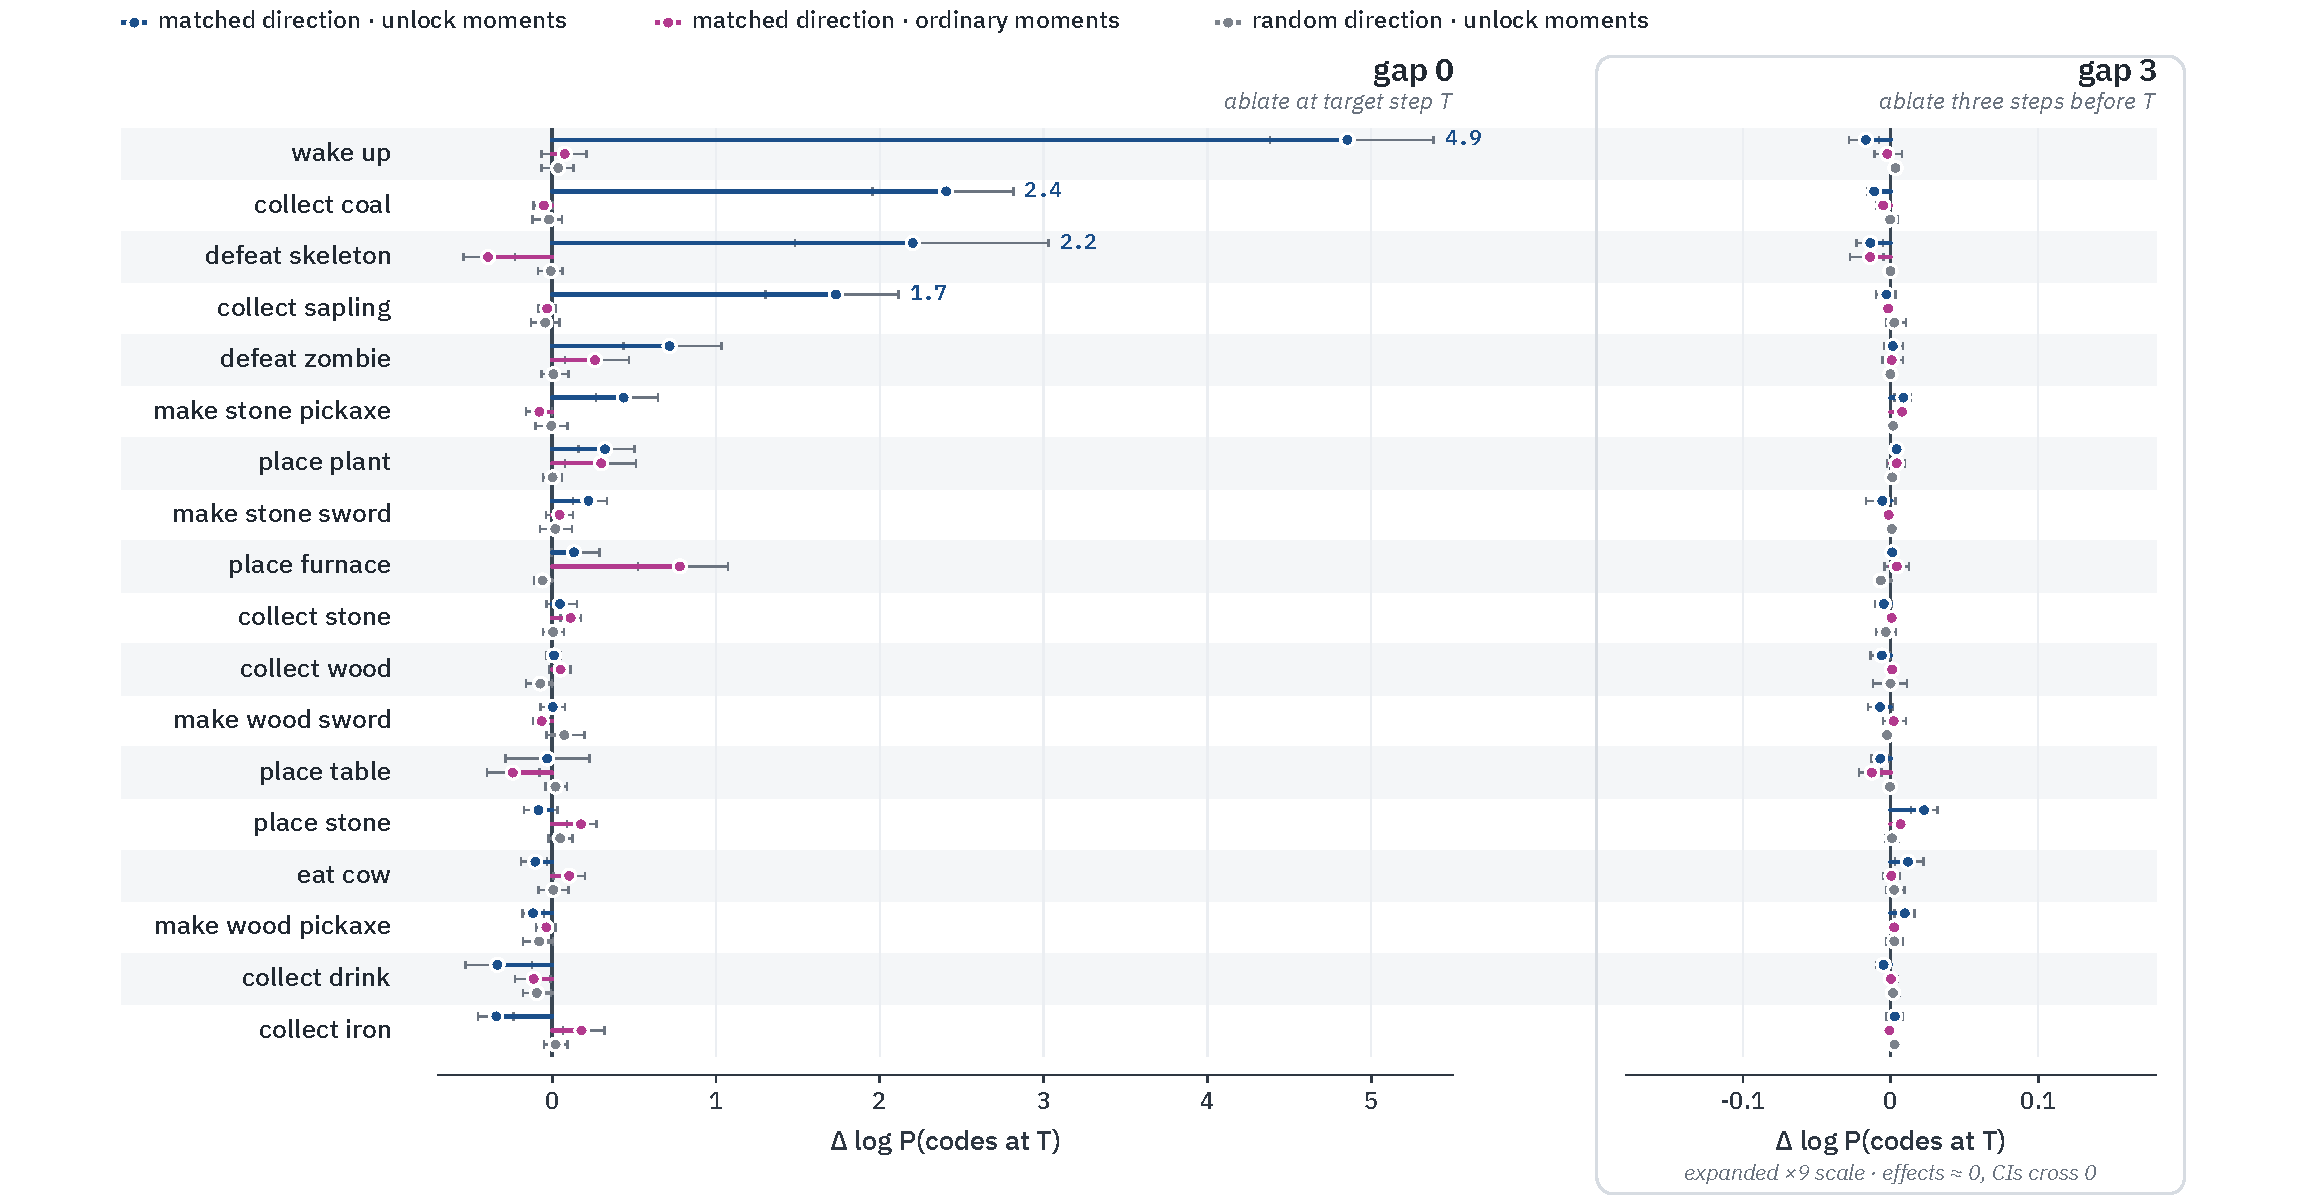
\includegraphics[width=\textwidth]{figures/ablation_onestep.pdf}
\caption{\textbf{Single-step causal ablation.} $\Delta\log P =$ baseline $-$ ablated log-likelihood of the four realised codes at the target step (positive $\Rightarrow$ ablation lowered their likelihood) when a direction is projected out of the block-1 residual stream, at the target step (gap~0, left) or three steps earlier (gap~3, right), on one shared horizontal scale. Markers are means; whiskers $95\%$ bootstrap CIs; the full $2\times2$ of \{matched, random\} direction $\times$ \{unlock, ordinary\} moment is shown. Random directions are inert; the matched direction is selective to unlock moments only for the dominant concepts; effects vanish entirely at gap~3 (the interventional face of the HUD shortcut).}\label{sfig:onestep}
\end{figure}

\begin{figure}[h]
\centering
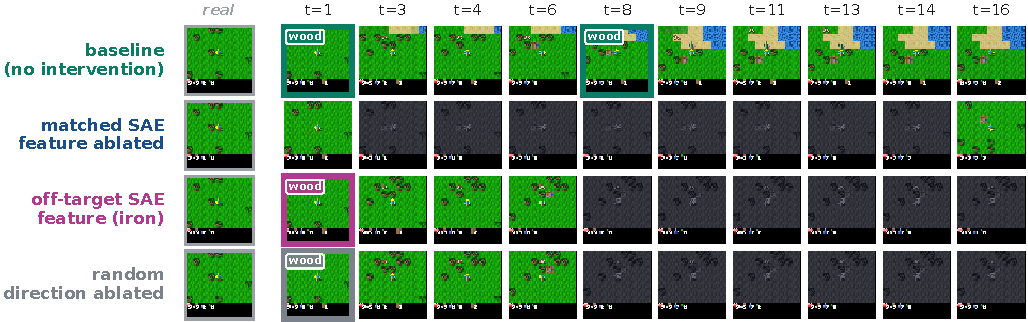
\includegraphics[width=\textwidth]{figures/filmstrip_headline.pdf}\\[6pt]
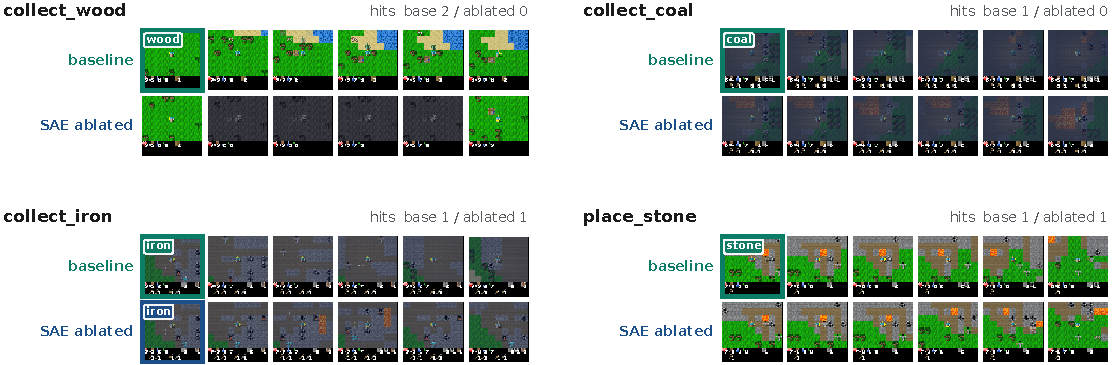
\includegraphics[width=\textwidth]{figures/filmstrip_grid.pdf}
\caption{\textbf{Imagined trajectories under ablation (decoded frames).} Top: paired trajectories for \achname{collect\_wood} from a shared burn-in and sampling seed---no intervention; matched SAE feature ablated (wood never appears, dream degrades); off-target SAE feature ablated (the \achname{collect\_iron} feature, a magnitude-comparable control); random unit direction. Only the matched direction erases the event. Bottom: baseline vs matched-SAE ablation for four concepts, ranging from clean erasure (\achname{collect\_wood}) through partial suppression (\achname{collect\_coal}) to none (\achname{collect\_iron}, \achname{place\_stone})---honest negatives whose best SAE features are not causally load-bearing.}\label{sfig:film}
\end{figure}

\begin{figure}[h]
\centering
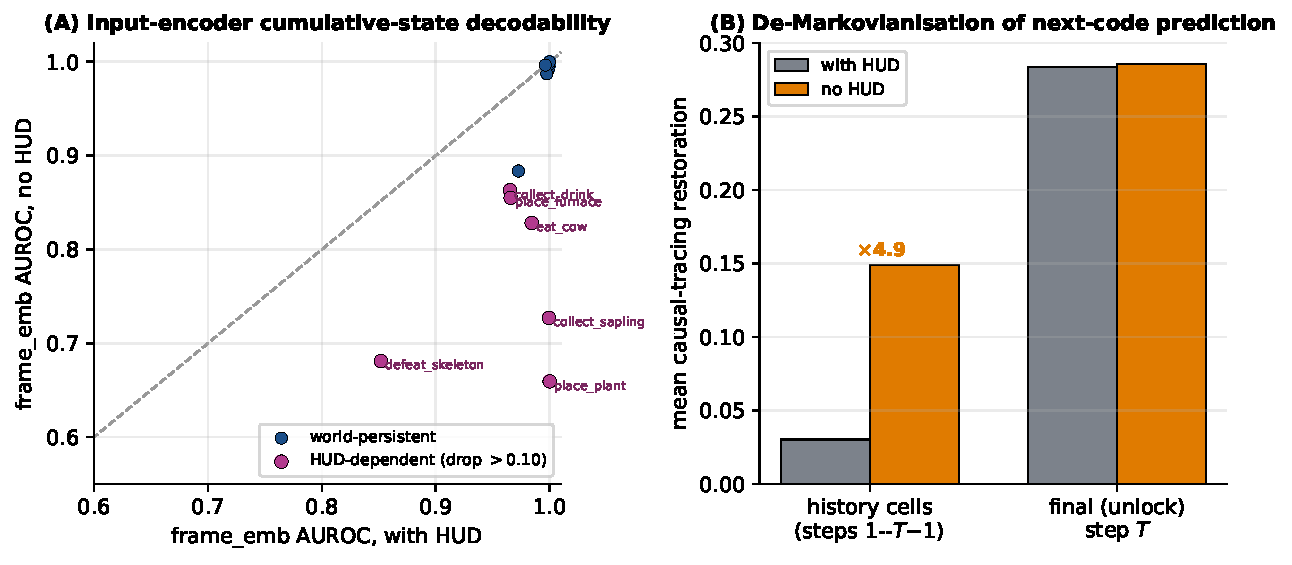
\includegraphics[width=\textwidth]{figures/nohud_compare.pdf}
\caption{\textbf{Partially observed (no-HUD) control: with-HUD vs no-HUD.} A second agent (identical code, hyperparameters and seed) was trained on a Crafter variant that zeroes the on-screen inventory/vitals region; mean return falls from $16.2$ to $9.7$. \textbf{(A)} input-encoder (\textsf{frame\_emb}) held-out AUROC for each cumulative-state concept, with HUD ($x$) vs no-HUD ($y$). World-persistent achievements (blue; placed objects, gathered materials, tools) stay near $1.0$ because they leave visible marks in the scene, so the input-encoder shortcut survives; only the six genuinely HUD-only concepts (magenta) drop below the diagonal. A transformer block out-reads \textsf{frame\_emb} on only $1$ of $17$ concepts, so the hidden state is not made linearly decodable from the blocks. \textbf{(B)} causal-tracing restoration mass on history cells (steps $1$ to $T{-}1$) vs the final unlock step: with state hidden, mean historical restoration rises $\approx\!5\times$ ($0.03\to0.15$) while the final-step mass is unchanged---next-code prediction de-Markovianises.}\label{sfig:nohud}
\end{figure}

\begin{figure}[h]
\centering
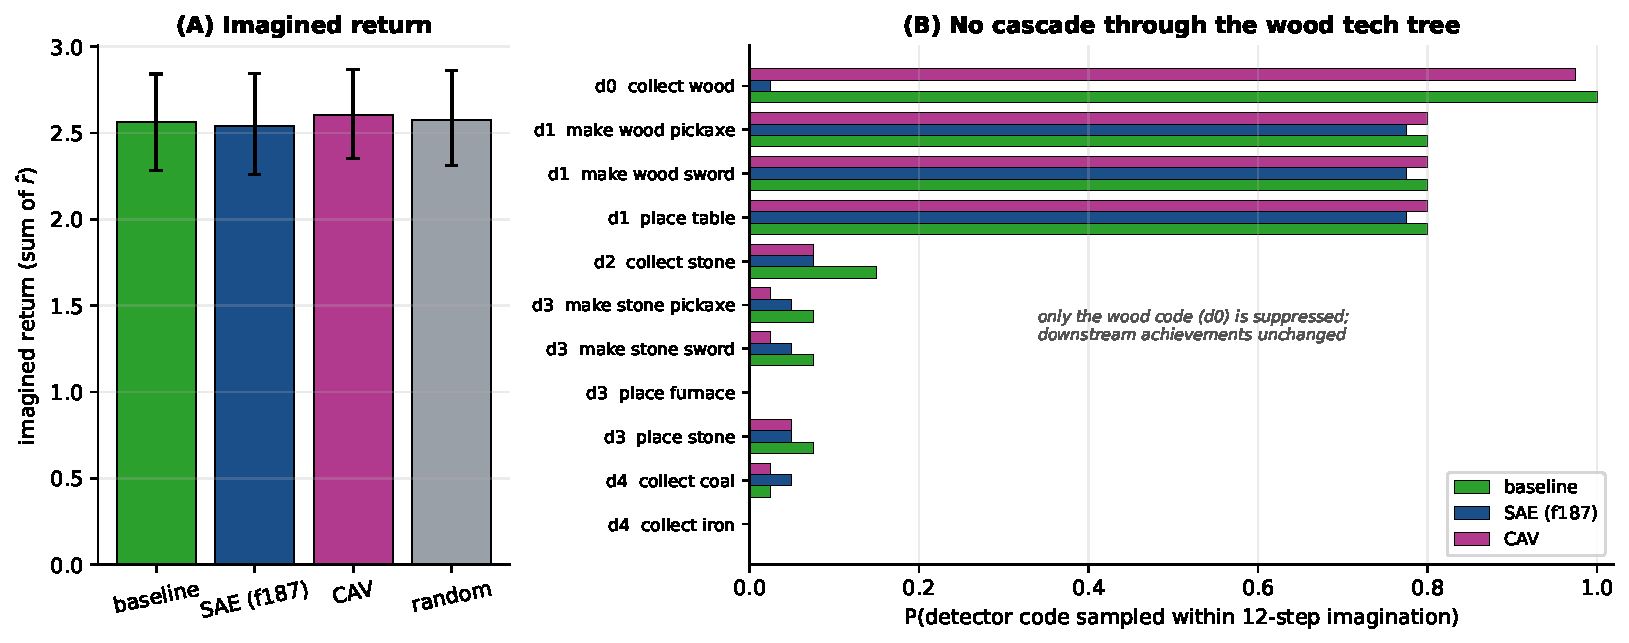
\includegraphics[width=\textwidth]{figures/cascade.pdf}
\caption{\textbf{Behavioural cascade test: a residual-stream lesion of the \achname{collect\_wood} feature ($f_{187}$) does not change the agent's imagined behaviour.} Closed-loop imagination from \achname{collect\_wood} unlock moments ($n{=}40$; the actor--critic acts on each decoded frame), under baseline / SAE-$f_{187}$ / wood-CAV / random projection at block~1. \textbf{(A)} imagined return (sum of the reward head) is unchanged across conditions ($2.56$, $2.54$, $2.61$, $2.58$). \textbf{(B)} per wood-tree achievement, ordered by tech-tree depth from \achname{collect\_wood}, the probability its detector code is sampled within the 12-step horizon. Ablating $f_{187}$ erases only the wood code itself (depth 0, $1.00\to0.03$) and does \emph{not} cascade: the immediately downstream wooden-tool achievements (depth 1; sampled via the shared polysemantic code $\code{3}{36}$) and the stone tier are unchanged, and the CAV and random directions are equally inert. The SAE direction is causally load-bearing for the next-code distribution but behaviourally inert---it does not propagate through the tech tree---corroborating, with a ground-truth causal graph, that the read--write effect is confined to the code channel.}\label{sfig:cascade}
\end{figure}

\begin{figure}[h]
\centering
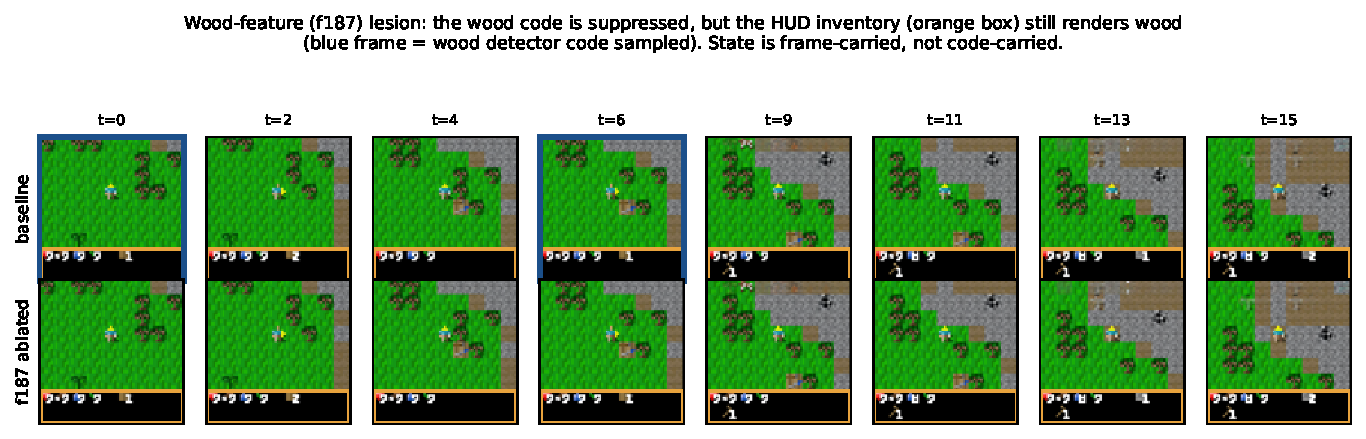
\includegraphics[width=\textwidth]{figures/hud_smoking_gun.pdf}
\caption{\textbf{Why the write does not drive: the suppressed state is carried by the frame, not the code.} Paired decoded imagination for a \achname{collect\_wood} moment, baseline (top) vs wood-feature ($f_{187}$) ablation (bottom); the orange box marks the HUD inventory/vitals strip (rows $y\ge 49$), a blue frame marks a step where the wood detector code is sampled. Under ablation the wood code is never sampled (blue frames vanish), yet the HUD inventory strip still renders the wood the agent holds: its mean per-pixel change from baseline is only $2.2/255$, versus $20.4/255$ ($\approx\!9.4\times$) in the world region above. Because the convolutional encoder re-reads the inventory from each frame, the downstream wooden-item codes can fire from this frame-carried state that the suppressed code never gated---the mechanism behind the powered behavioural null in Fig.~\ref{sfig:cascade}.}\label{sfig:hud}
\end{figure}

\clearpage
% ---------------- Supplementary Tables ----------------
\begin{table}[h]
\centering
\caption{\textbf{Strongest detector code per achievement} (selection). $n_{\mathrm{co}}$: co-occurrences of the code with the just-unlocked event; $n_c$: total occurrences; lift $=P(u\mid c)/P(u)$. All $p$-values are below $10^{-40}$ (uncorrected exact binomial); the full 431-cell table ships with the code release.}\label{stab:mi}
\begin{tabular}{@{}llrrr@{}}
\toprule
Achievement & Code & $n_{\mathrm{co}}/n_c$ & $P(u \mid c)$ & Lift \\
\midrule
\achname{place\_plant}        & $\code{3}{938}$ & $477/519$  & $0.92$ & $543\times$ \\
\achname{collect\_sapling}    & $\code{2}{707}$ & $419/463$  & $0.90$ & $535\times$ \\
\achname{collect\_iron}       & $\code{3}{75}$  & $360/410$  & $0.88$ & $708\times$ \\
\achname{collect\_coal}       & $\code{3}{578}$ & $450/626$  & $0.72$ & $467\times$ \\
\achname{make\_wood\_pickaxe} & $\code{3}{903}$ & $19/35$    & $0.54$ & $325\times$ \\
\achname{place\_table}        & $\code{3}{36}$  & $480/1507$ & $0.32$ & $188\times$ \\
\achname{eat\_cow}            & $\code{2}{648}$ & $251/1127$ & $0.22$ & $134\times$ \\
\achname{place\_furnace}      & $\code{0}{51}$  & $89/412$   & $0.22$ & $132\times$ \\
\achname{collect\_wood}       & $\code{3}{940}$ & $474/2471$ & $0.19$ & $113\times$ \\
\achname{defeat\_zombie}      & $\code{1}{727}$ & $68/365$   & $0.19$ & $113\times$ \\
\bottomrule
\end{tabular}
\end{table}

\begin{table}[h]
\centering
\caption{\textbf{Cross-corroborated SAE features.} The feature's top achievement (lift within its top activation quartile), most-aligned CAV, and the (slot, code) with the highest conditional mean activation. The first five satisfy strict triple-corroboration ($|\cos|>0.4$ to the same-named CAV); $f_{372}$ is the third member of the $\code{3}{36}$ split.}\label{stab:sae}
\begin{tabular}{@{}llll@{}}
\toprule
Feature & Achievement (lift) & CAV ($\cos$) & Code \\
\midrule
$f_{1742}$ & \achname{collect\_coal} ($589\times$) & just[\achname{collect\_coal}] ($+0.58$) & $\code{3}{578}$ \\
$f_{1820}$ & \achname{collect\_iron} ($624\times$) & just[\achname{collect\_iron}] ($+0.41$) & $\code{3}{75}$ \\
$f_{872}$  & \achname{make\_stone\_pickaxe} ($522\times$) & just[\achname{make\_stone\_pickaxe}] ($+0.48$) & $\code{3}{616}$ \\
$f_{677}$  & \achname{place\_table} ($527\times$) & just[\achname{place\_table}] ($+0.45$) & $\code{3}{36}$ \\
$f_{1451}$ & \achname{make\_wood\_pickaxe} ($548\times$) & just[\achname{make\_wood\_pickaxe}] ($+0.46$) & $\code{3}{36}$ \\
$f_{372}$  & \achname{make\_wood\_sword} ($444\times$) & just[\achname{make\_wood\_sword}] ($+0.23$) & $\code{3}{36}$ \\
\bottomrule
\end{tabular}
\end{table}

\begin{table}[h]
\centering
\caption{\textbf{Matched-protocol reconstruction} on a common $8{,}192$-transition held-out batch. Perplexity is $\exp(\text{entropy})$ of the token histogram over all slots. \deltairis{} conditions its decoder on $(x_t,a_t)$; the baselines reconstruct $x_{t+1}$ from codes alone, so \deltairis{}'s lower error is expected and not a like-for-like comparison.}\label{stab:recon}
\begin{tabular}{@{}lrrrrr@{}}
\toprule
Tokenizer & MSE $\downarrow$ & PSNR $\uparrow$ & LPIPS $\downarrow$ & perplexity & tokens/frame \\
\midrule
\deltairis{} (delta + action) & $0.00021$ & $36.7$ & $0.048$ & $80.7$ & 4 \\
frame-only ablation           & $0.0145$  & $18.4$ & $0.467$ & $48.5$ & 4 \\
original IRIS                  & $0.0056$  & $22.5$ & $0.080$ & $109.2$ & 16 \\
\bottomrule
\end{tabular}
\end{table}

\begin{table}[h]
\centering
\caption{\textbf{HUD-shortcut margins with bootstrap CIs.} For each cumulative-state concept, \textsf{frame\_emb} held-out AUROC and the \emph{worst} (smallest) AUROC difference against any transformer block, with a paired-bootstrap $95\%$ CI ($B{=}1000$). \textsf{frame\_emb} is not significantly below any block on 16 of 18 concepts; the two exceptions (\achname{collect\_sapling}, \achname{place\_plant}) trail by $<10^{-3}$, with all representations above $0.999$.}\label{stab:hud}
\begin{tabular}{@{}lrrcc@{}}
\toprule
Concept & \textsf{frame\_emb} AUROC & worst $\Delta$AUROC & $95\%$ CI & not below \\
\midrule
\achname{collect\_coal}        & $1.000$ & $+0.046$ & $[+0.043,+0.049]$ & yes \\
\achname{collect\_drink}       & $0.965$ & $+0.046$ & $[+0.040,+0.051]$ & yes \\
\achname{collect\_iron}        & $1.000$ & $+0.065$ & $[+0.061,+0.068]$ & yes \\
\achname{collect\_sapling}     & $0.999$ & $-0.0007$ & $[-0.0010,-0.0004]$ & no \\
\achname{collect\_stone}       & $0.999$ & $+0.014$ & $[+0.013,+0.016]$ & yes \\
\achname{collect\_wood}        & $1.000$ & $+0.0015$ & $[+0.0010,+0.0020]$ & yes \\
\achname{defeat\_skeleton}     & $0.852$ & $+0.009$ & $[+0.004,+0.013]$ & yes \\
\achname{defeat\_zombie}       & $0.973$ & $+0.019$ & $[+0.016,+0.022]$ & yes \\
\achname{eat\_cow}             & $0.984$ & $+0.012$ & $[+0.009,+0.015]$ & yes \\
\achname{make\_stone\_pickaxe} & $1.000$ & $+0.018$ & $[+0.016,+0.019]$ & yes \\
\achname{make\_stone\_sword}   & $1.000$ & $+0.020$ & $[+0.018,+0.022]$ & yes \\
\achname{make\_wood\_pickaxe}  & $1.000$ & $+0.008$ & $[+0.007,+0.009]$ & yes \\
\achname{make\_wood\_sword}    & $1.000$ & $+0.042$ & $[+0.039,+0.046]$ & yes \\
\achname{place\_furnace}       & $0.966$ & $+0.015$ & $[+0.012,+0.019]$ & yes \\
\achname{place\_plant}         & $1.000$ & $-0.0000$ & $[-0.0000,-0.0000]$ & no \\
\achname{place\_stone}         & $0.997$ & $+0.017$ & $[+0.015,+0.018]$ & yes \\
\achname{place\_table}         & $0.996$ & $+0.016$ & $[+0.013,+0.018]$ & yes \\
\achname{wake\_up}             & $0.916$ & $+0.034$ & $[+0.029,+0.041]$ & yes \\
\bottomrule
\end{tabular}
\end{table}

\begin{table}[h]
\centering
\caption{\textbf{Sparse-autoencoder robustness sweep} on the block-1 summary activations ($81{,}919$ samples, 60 epochs), and single SAEs at other layers. FVU: fraction of variance unexplained on episode-disjoint validation. Detector features reappear as each variant's own top detector (mean matched decoder cosine $0.63$).}\label{stab:saegrid}
\begin{tabular}{@{}llrr@{}}
\toprule
Axis & Config ($M$, $k$, seed / layer) & FVU & dead features \\
\midrule
width      & $1024$, $16$, $0$  & $0.0445$ & $0$ \\
(default)  & $2048$, $16$, $0$  & $0.0440$ & $0$ \\
width      & $4096$, $16$, $0$  & $0.0441$ & $0$ \\
sparsity   & $2048$, $8$, $0$   & $0.0543$ & $28$ \\
sparsity   & $2048$, $32$, $0$  & $0.0363$ & $0$ \\
seed       & $2048$, $16$, $1$  & $0.0439$ & $0$ \\
\midrule
layer      & \textsf{frame\_emb} & $0.267$  & --- \\
layer      & \textsf{wm\_input}  & $0.0475$ & --- \\
layer      & \textsf{block\_2}   & $0.0265$ & --- \\
layer      & \textsf{block\_3}   & $0.214$  & --- \\
\bottomrule
\end{tabular}
\end{table}

\begin{table}[h]
\centering
\caption{\textbf{Empirical random-direction null.} Single-step matched-SAE ablation effect (gap~0) against an $R{=}50$ random-direction null; $z=(\text{matched}-\mu_{\text{null}})/\sigma_{\text{null}}$. The matched effect clears the $99$th percentile for three of eight dominant concepts; honest negatives (e.g.\ \achname{collect\_iron}) sit at or below the null.}\label{stab:null}
\begin{tabular}{@{}lrrrc@{}}
\toprule
Concept & matched $\Delta\log P$ & null $\mu\pm\sigma$ & $z$ & $>p_{99}$ \\
\midrule
\achname{collect\_coal}        & $+2.70$ & $-0.02\pm0.11$ & $24.2$ & yes \\
\achname{collect\_sapling}     & $+1.73$ & $+0.02\pm0.17$ & $9.9$  & yes \\
\achname{make\_stone\_pickaxe} & $+0.61$ & $-0.01\pm0.20$ & $3.1$  & yes \\
\achname{place\_plant}         & $+0.32$ & $+0.02\pm0.21$ & $1.4$  & no \\
\achname{make\_wood\_pickaxe}  & $-0.16$ & $-0.01\pm0.15$ & $-1.0$ & no \\
\achname{place\_table}         & $-0.04$ & $-0.04\pm0.20$ & $0.0$  & no \\
\achname{place\_stone}         & $-0.11$ & $-0.03\pm0.19$ & $-0.5$ & no \\
\achname{collect\_iron}        & $-0.39$ & $-0.02\pm0.16$ & $-2.3$ & no \\
\bottomrule
\end{tabular}
\end{table}

\begin{table}[h]
\centering
\caption{\textbf{Steering (sufficiency) inside imagination.} Adding the matched SAE direction ($h\mathrel{+}=\alpha\hat d$) from ordinary moments raises within-horizon detector-code probability only weakly; suppression (matched ablation) is shown for comparison. Mean induction gain $+0.04$ vs suppression drop $+0.07$ across 12 concepts (mean activate$-$suppress $=-0.03$): no activate-over-suppress asymmetry in this agent.}\label{stab:steer}
\begin{tabular}{@{}lrrrr@{}}
\toprule
Concept & induce base & induce gain & suppress base & suppress drop \\
\midrule
\achname{collect\_sapling}     & $0.00$ & $+0.25$ & $0.60$ & $+0.20$ \\
\achname{collect\_stone}       & $0.15$ & $+0.20$ & $1.00$ & $+0.00$ \\
\achname{collect\_iron}        & $0.05$ & $+0.05$ & $1.00$ & $+0.15$ \\
\achname{make\_stone\_pickaxe} & $0.10$ & $+0.05$ & $0.80$ & $+0.10$ \\
\achname{place\_stone}         & $0.05$ & $+0.05$ & $1.00$ & $+0.00$ \\
\achname{collect\_coal}        & $0.05$ & $-0.05$ & $0.95$ & $+0.25$ \\
\achname{eat\_cow}             & $0.15$ & $-0.05$ & $0.75$ & $+0.00$ \\
\achname{make\_stone\_sword}   & $0.10$ & $+0.00$ & $0.75$ & $+0.30$ \\
\achname{wake\_up}             & $0.00$ & $+0.00$ & $0.30$ & $-0.20$ \\
\bottomrule
\end{tabular}
\end{table}

\begin{table}[h]
\centering
\caption{\textbf{Direct logit attribution} to the detector code, mean over 18 concepts ($n{=}40$ unlock moments each). $\overline{|\text{det}|}$: mean absolute attribution to the detector code; $\overline{|\text{det}|-|\text{ctrl}|}$: detector-vs-control specificity; \#sig: concepts whose detector attribution CI excludes 0. The SAE direction's attribution is $\sim\!4\times$ the CAV's and $\sim\!24\times$ a random direction's; the sign is concept-dependent (off-path \achname{collect\_iron} $-1.56$, \achname{wake\_up} $+1.50$).}\label{stab:logit}
\begin{tabular}{@{}lrrr@{}}
\toprule
Direction & $\overline{|\text{det}|}$ & $\overline{|\text{det}|-|\text{ctrl}|}$ & \#sig / 18 \\
\midrule
SAE feature & $0.311$ & $+0.073$ & $9$ \\
CAV         & $0.083$ & $+0.024$ & $6$ \\
random      & $0.013$ & $+0.000$ & $2$ \\
\bottomrule
\end{tabular}
\end{table}

\end{document}
